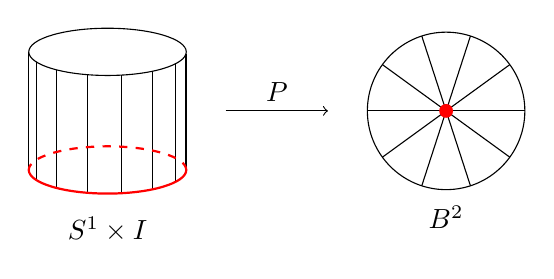
\begin{tikzpicture}
\draw (0,1.5) ellipse (1 and 0.3);
\foreach \a in {180,205,...,360} \draw (\a:1 and 0.3) -- ++(0,1.5);
\draw[red, thick] (-1,0) arc (180:360:1 and 0.3);
\draw[red, thick, dashed] (1,0) arc (0:180:1 and 0.3);
\node at (0,-0.75) {$S^1\times I$};
\draw[->] (1.5,0.75) -- node[above] {$P$} (2.8,0.75);
\draw (4.3,0.75) circle (1);
\foreach \a in {0,36,...,324} \draw (4.3,0.75) -- ++(\a:1);
\fill[red] (4.3,0.75) circle (2.5pt);
\node at (4.3,-0.6) {$B^2$};
\end{tikzpicture}
